\section{Felhasználói felület}
\subsection{Főoldal}
A weboldalra rákeresve a felhasználót a kezdőoldal fogadja, ahol lehetőség van
egy utazás megtervezésére. Ki kell választani a kiindulási helyet és megállót, majd a
célt, az utazás dátumát és időpontját. Ekkor a rendszer lekéri a szerverről a megadott
megállók közötti, az adott napon, a megadott időpont után közlekedő járatokat és azok
jegyárát. Minden egyes járatnál van egy vásárlás gomb, amellyel a felhasználó
megszerezheti a jegyet vagy jegyeit az adott buszjáratra, amennyiben be van
jelentkezve, ellenkező esetben a rendszer átirányítja a bejelentkezéshez.

\begin{figure}[H]
    \centering
    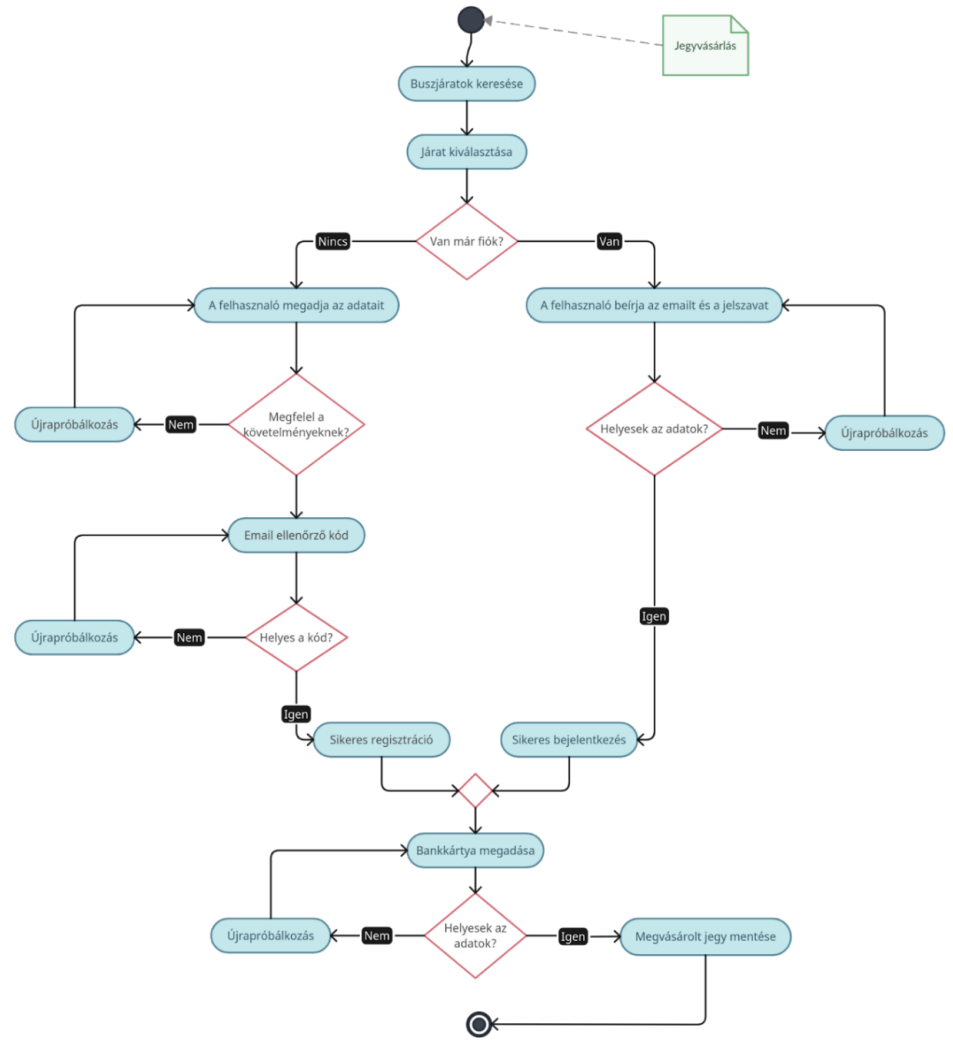
\includegraphics[width=\textwidth]{figures/activity.png}
    \caption{Aktivitás diagram az utazás tervezésének folyamatáról}
    \label{fig:activity-diagram}
\end{figure}

Ahogy a \ref{fig:activity-diagram} ábrán is látható, miután a felhasználó megtalálta a megfelelő
buszjáratot és rálépett a jegy(ek) megvásárlására, a rendszer átirányítja őt a
bejelentkezéshez, itt ha van már fiókja, bejelentkezhet a meglévő adataival,
amennyiben nincs, úgy átléphet a regisztrációs oldalra, ahol meg kell adnia a nevét,
email címét, és egy új jelszót. A rendszer minden adatot ellenőriz és ha valamelyik
hibás (pl. érvénytelen email cím vagy túl rövid jelszó) akkor egy hibaüzenetet ír ki. Ez
addig ismétlődik, amíg minden adat megfelelő lesz, aztán automatikusan küldünk egy
ellenőrző kódot a megadott e-mailre, amelyet a felhasználó be kell írjon a webes
felületen megjelenő szövegmezőbe.

\begin{figure}[H]
    \centering
    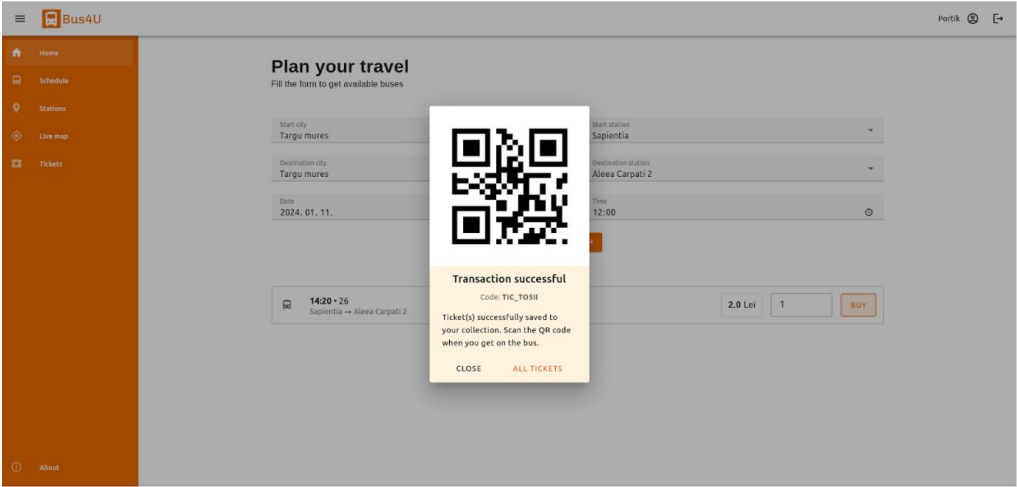
\includegraphics[width=\textwidth]{figures/boughtticket.png}
    \caption{Megvásárolt jegy}
    \label{fig:bought-ticket}
\end{figure}

Ha ez helytelen, ez is addig ismétlődik, amíg
minden rendben lesz, majd a rendszer átirányítja a felhasználót a bankkártyás
fizetéses oldalra, ami jelenleg nincs implementálva, ez a jövőbeli tervek között
szerepel. Ezután már csak az következik, hogy a rendszer elmenti a megvásárolt jegy
kódját, amelyet a felhasználó a Jegyek oldalon talál meg szöveges és QR-kódos
formátumban.

\begin{figure}[H]
    \centering
    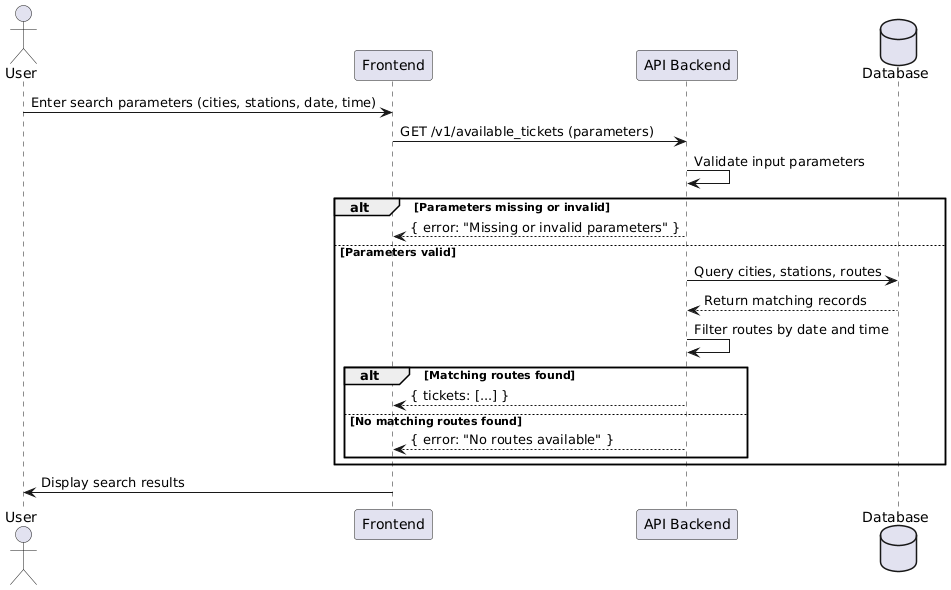
\includegraphics[width=\textwidth]{figures/listtickets.png}
    \caption{Szekvencia diagram az útvonaltervezés folyamatáról}
    \label{fig:seq-diagram-1}
\end{figure}

\subsection{Jegyek}
A megvásárolt jegyeket a rendszer elmenti a gyűjteménybe, ami a Jegyek oldalon
található, így a jegyek bármikor visszakereshetőek és felhasználhatóak lesznek,
kivéve ha lejár az egy hónapos érvényesség.

A jegyen megjelenített adatok között van
a járat neve, a kiinduló- és célállomás, az ár, valamint a vásárlás és az érvényesség
dátumai. A már elhasznált jegyek megvannak jelölve így azokat nem lehet többször
felhasználni.
A jegyeket QR-kód formájában is megjelenítjük ( \ref{fig:bought-ticket} ábra), amelyeket az utasok be tudnak szkennelni.

\begin{figure}[H]
    \centering
    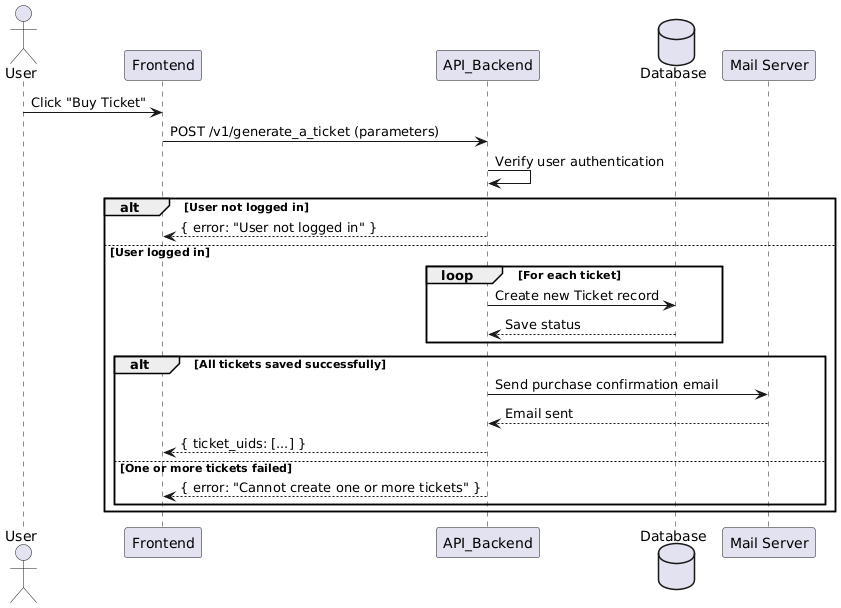
\includegraphics[width=\textwidth]{figures/buyticket.png}
    \caption{Szekvencia diagram a jegyvásárlás folyamatáról}
    \label{fig:seq-diagram-2}
\end{figure}

\subsection{Menetrend}
A következő oldal a menetrend, amely hasonlóan a buszmegállókban kihelyezett
táblázatokhoz, megjeleníti a kiválasztott buszjárat indulási időpontjait, az adott
megállóból. A mi megoldásunk viszont tartalmaz emellett egy térképet is, ahol meg
lehet nézni a járat útvonalát, az érintett megállókat és az útvonalon közlekedő buszok
élő pozícióját is.

\subsection{Megállók és térkép}
Ez a két oldal a fent említett térképes funkciókat mutatják meg külön-külön,
egyszerűbben. Egyik megjeleníti a térképen az összes megállót, és ezek között
szűrést is biztosít város vagy buszjárat szerint. A másik oldalon pedig egy-egy
útvonalon közlekedő buszok élő pozícióját lehet követni, miután kiválasztottuk a várost
és az útvonalat. Ez a funkció abban segít, hogy ne maradjunk le, ha egy busz siet,
illetve ne várakozzunk feleslegesen a megállóban, ha egy busz késik, így időt lehet
vele spórolni.

\section{Adminisztrációs felület}
Az admin felület csak bejelentkezéssel elérhető, ehhez egy admin rangú
felhasználói fiók szükséges, amely egy adott céghez van hozzárendelve. A cégek
adatai el vannak különítve, így minden admin csak a saját cégéhez tartozó adatokat
láthatja és módosíthatja.

\subsection{Kezdőlap}
Belépés után egy összegző oldal jelenik meg amelyen látható egy kis statisztika
a regisztrált felhasználók számával, a megvásárolt jegyek számával és a bevétellel,
mindez havi, évi és mindenkori bontásban. Itt jelennek meg az esetleges
figyelmeztetések és értesítések is, például a buszok lejárt útadója vagy a közelgő
műszaki vizsgálat.

\begin{figure}[H]
    \centering
    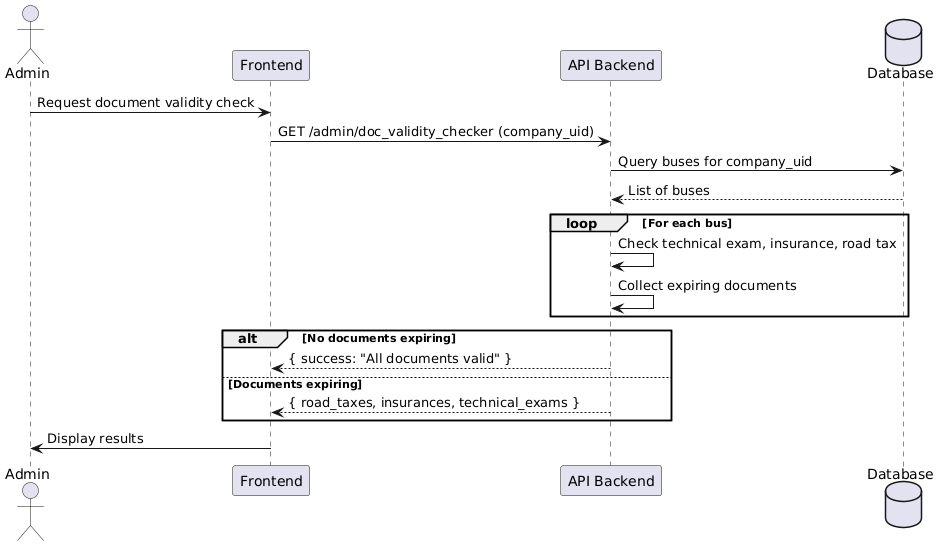
\includegraphics[width=\textwidth]{figures/checkdocuments.png}
    \caption{Szekvencia diagram a dokumentumok ellenőrzéséről}
    \label{fig:seq-diagram-3}
\end{figure}

\subsection{Megállók}
A Megállók oldalon létre lehet hozni új megállókat, megtekinteni meglévőket a
térképen vagy törölni ezeket. Új megálló hozzáadásához meg kell adni a megálló
nevét, a címet és a koordinátákat. A néven kívül, a többi adatot automatikusan kitölti a
rendszer, ha a térképen a megálló helyére kattint a felhasználó, de manuálisan is meg
lehet adni.

\subsection{Útvonalak}
Ezen az oldalon lehet felépíteni útvonalakat a létrehozott megállókból és itt lehet
megadni az alap jegyárat is, abban az esetben, ha a jegyek ára nem függ a megtett
távolságtól és időtől, hanem mindig és mindenhova ugyanannyi, ez esetben a fizetés
az útvonalhoz lesz hozzárendelve, nem a különböző megállókhoz.

\subsection{Menetrend}
A következő oldal a Menetrend, ahol a létrehozott útvonalak megállóihoz lehet
órarendeket hozzárendelni. Itt meg kell adni az órarendre érvényes napokat, a
következő megállóig szükséges jegyárat és az indulási időpontokat. Egy megállóhoz
hozzá lehet adni több ilyen órarendet is, ha különböző napokra különböző órarend
érvényes. Így el lehet választani a hétvégét a hétköznapoktól, ha mások az indulási
időpontok, vagy ha például hétvégén drágább a jegy.

\subsection{Buszok és alkalmazottak}
Az utolsó két oldalon a buszokat és az alkalmazottakat lehet kezelni. Hasonlóan
működnek, mindkettőn található egy lista a meglévő elemekkel, ahol bármelyiket lehet
módosítani vagy törölni, illetve újat is lehet létrehozni. A buszoknál meg kell adni a
márkát, a rendszámot, a férőhelyek számát, a gyártási évet, valamint az útadó, a
biztosítás és a műszaki engedély lejárati dátumát. Új alkalmazott hozzáadásánál meg
kell adni a nevet, e-mail címet, beosztást, telefonszámot, lakcímet (opcionális), és egy
új jelszavat.


\section{POS terminál alkalmazása}
\subsection{GPS oldal}
Miután a sofőr bejelentkezett, ezen
az oldalon lehetőség nyílik kiválasztani
az aktuális buszt, amelyiket jelenleg a
sofőr vezet, illetve azt az útvonalat,
amelyet éppenséggel végrehajt. Található egy kapcsoló, amellyel el lehet
indítani az autóbusz lokációjának
követését. Ez félpercenként küldi fel az
API-ra a busz lokációját, ezáltal lehet a
weboldalon és az alkalmazásban élőben
követni a busz helyzetét. Illetve ezen opció bekapcsolásakor megjelenik egy térkép is, amelyen élőben láthatjuk a busz pontos helyzetét.
Legalul egy Ticket scanner gomb fedezhető fel,
amely átirányít a jegyszkennelő oldalra

\begin{figure}[H]
    \centering
    \begin{minipage}{0.48\textwidth}
        \centering
        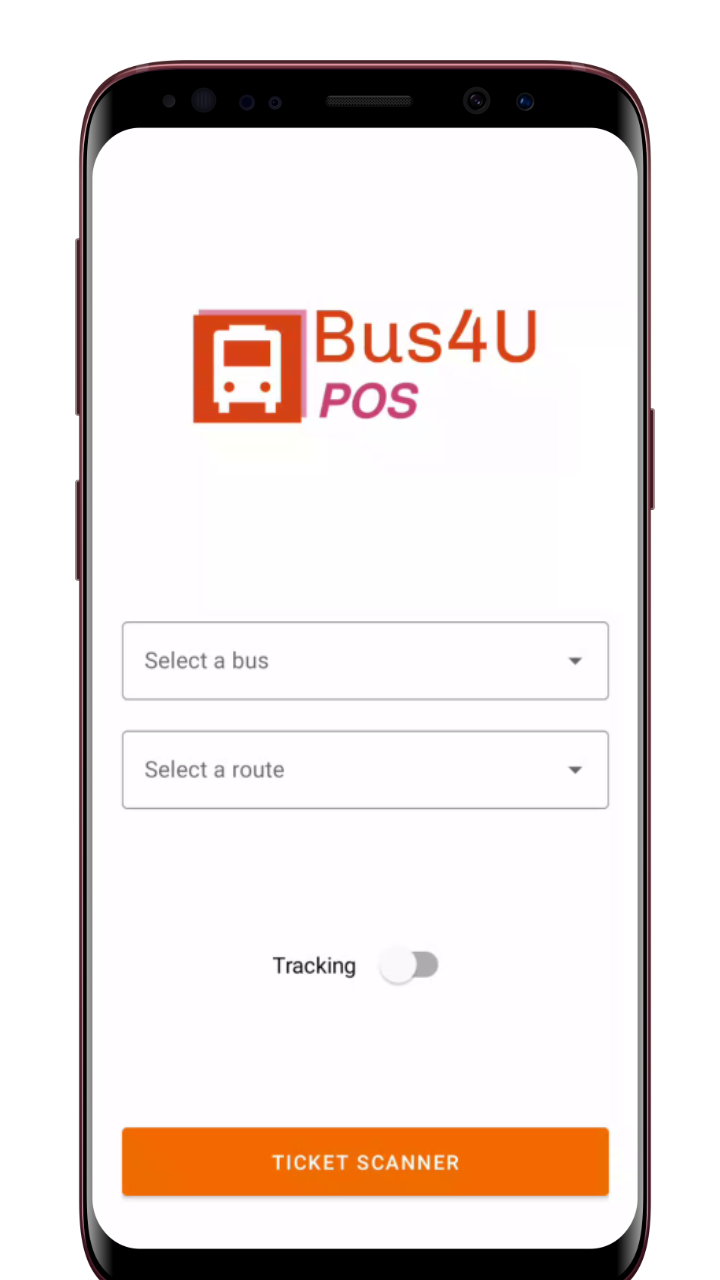
\includegraphics[width=\textwidth]{figures/pos_1.png}
        \caption{Busz kiválasztása és GPS követés}
        \label{fig:gps1}
    \end{minipage}\hfill
    \begin{minipage}{0.48\textwidth}
        \centering
        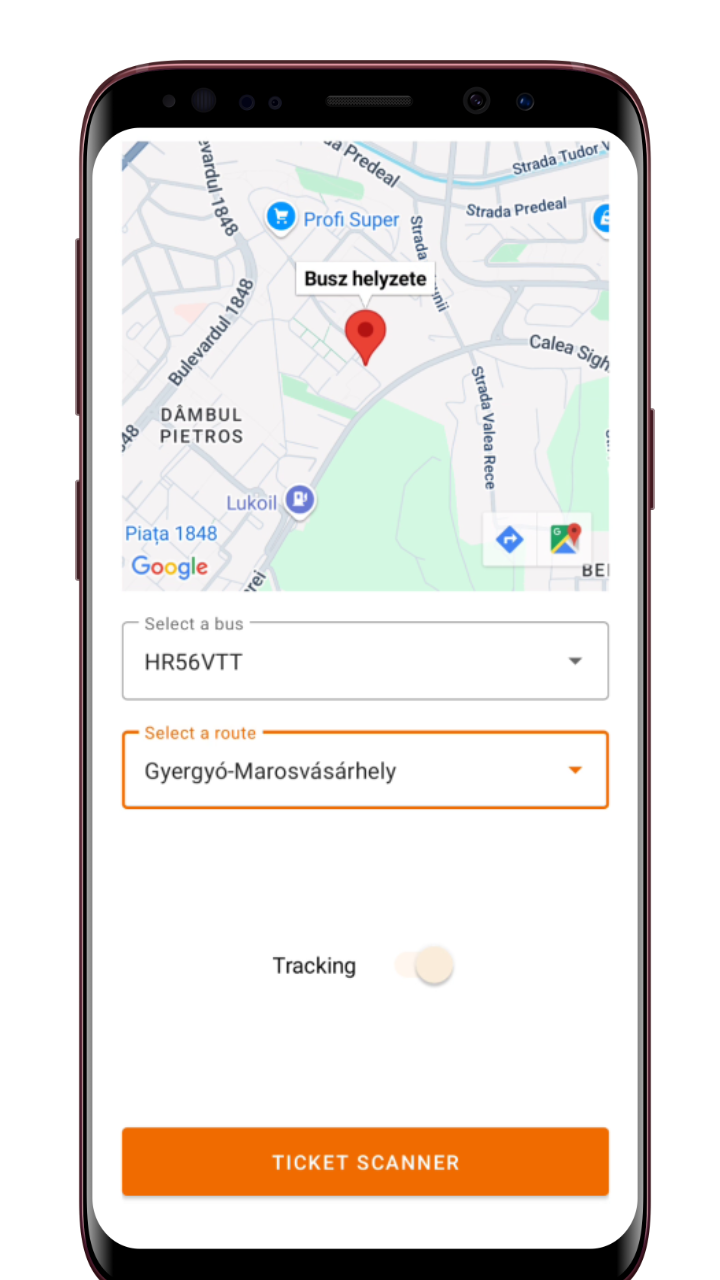
\includegraphics[width=\textwidth]{figures/pos_2.png}
        \caption{Elindított GPS követés}
        \label{fig:gps2}
    \end{minipage}
\end{figure}

\subsection{Jegyszkennelő oldal}
Ez az oldal a kamerát jeleníti meg.
Itt kell beszkennelni a jegyet. Szkennelés
után egy szöveges üzenet jelenik meg 5
másodpercig, három üzenetet hordozhat:
Ha sikeresen érvényesítve van a jegy,
akkor zöld háttérrel kiírja hogy sikeres
érvényesítés. Ha a jegy már érvényesítve
volt, vagy érvénytelen a QR kód, ezt egy
piros hibaüzenettel jelzi. Illetőleg ha az
API valamilyen oknál fogva leáll, akkor
ennek a hibájáról is üzenetet kapunk.

\begin{figure}[H]
    \centering
    \begin{minipage}{0.48\textwidth}
        \centering
        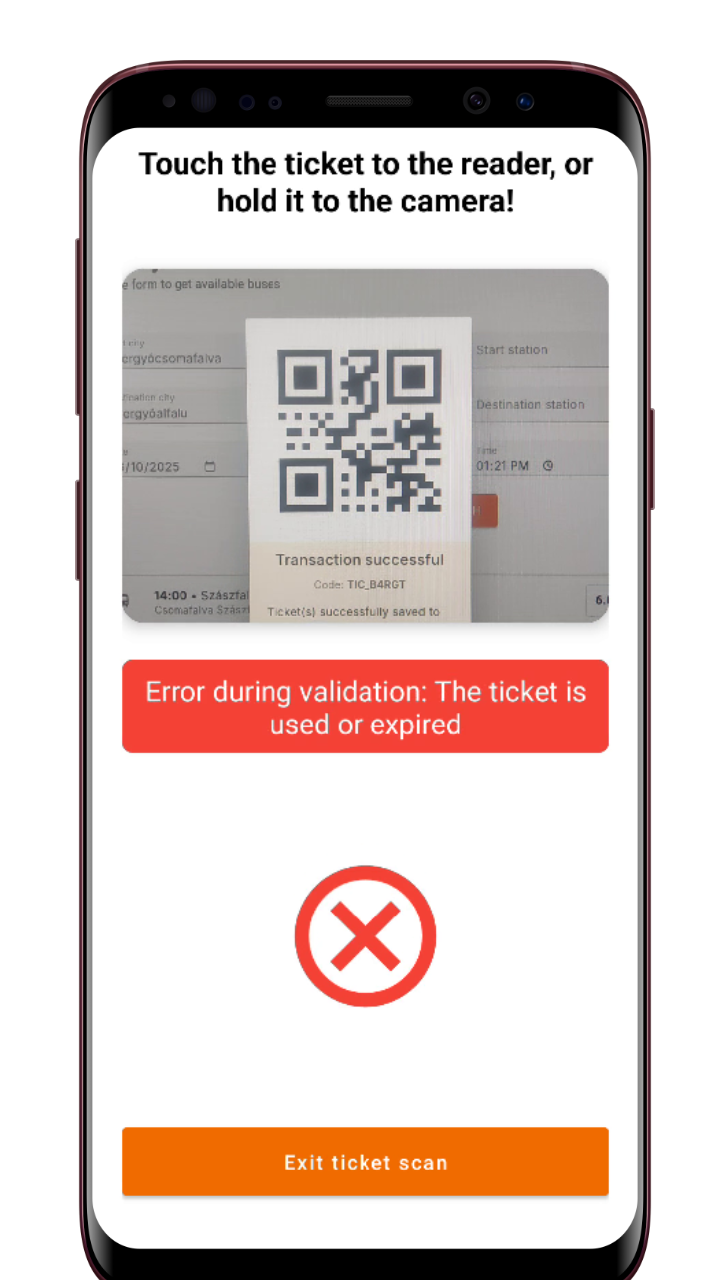
\includegraphics[width=\textwidth]{figures/pos_3.png}
        \caption{Sikeres jegy érvényesítés}
        \label{fig:pos_success}
    \end{minipage}\hfill
    \begin{minipage}{0.48\textwidth}
        \centering
        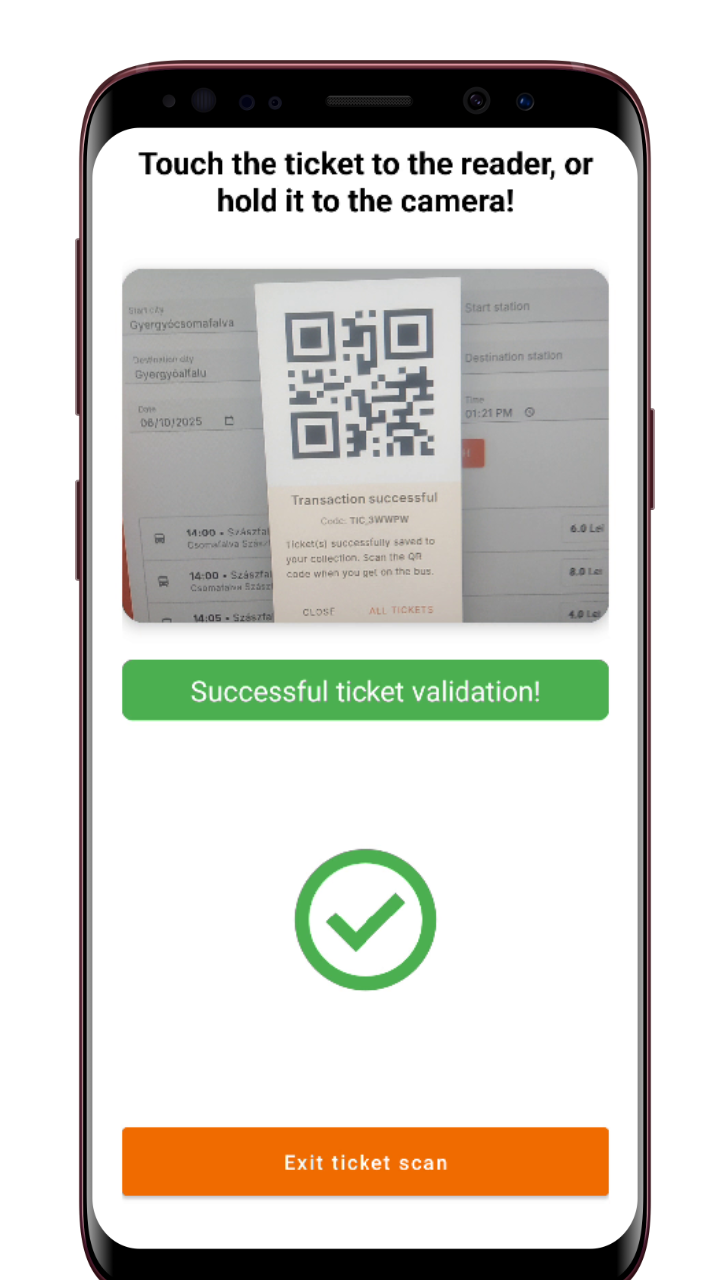
\includegraphics[width=\textwidth]{figures/pos_4.png}
        \caption{Sikertelen jegy érvényesítés}
        \label{fig:pos_error}
    \end{minipage}
\end{figure}